% First draft: 1958_guangdong_q9_solution_fig1 (exact: hypotenuse 2, altitude sqrt3/2).
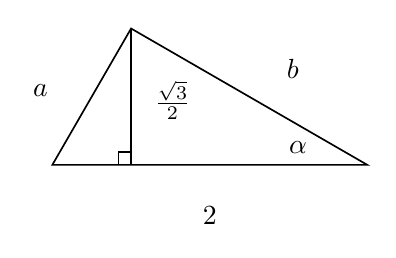
\begin{tikzpicture}[x=1cm,y=1cm,font=\normalsize,
 geometry edge/.style={solid,line width=.6pt},
 geometry mark/.style={solid,line width=.6pt},
 geometry label/.style={font=\normalsize,inner sep=2pt}]
\coordinate (L) at (0,0);
\coordinate (R) at (4,0);
\coordinate (T) at (1.000000000,1.732050808);
\coordinate (H) at (1,0);
\coordinate (L_a) at (0.02,0.95);
\coordinate (L_b) at (2.9,1.02);
\coordinate (L_alpha) at (3.120000000,0.220000000);
\coordinate (L_2) at (2,-0.45);
\coordinate (L_h) at (1.220000000,0.820000000);
\draw[geometry edge] (L)--(R)--(T)--cycle;
\draw[geometry edge] (T)--(H);
\draw[geometry mark] (0.84,0)--(0.84,0.16)--(1,0.16);
\node[geometry label,left] at (L_a) {$a$};
\node[geometry label,above right] at (L_b) {$b$};
\node[geometry label] at (L_alpha) {$\alpha$};
\node[geometry label,below] at (L_2) {$2$};
\node[geometry label,right] at (L_h) {$\frac{\sqrt{3}}{2}$};
\end{tikzpicture}
